%%%%%%%%%%%%%%%%%%%%%%%%%%%%%%%%%%%%%%%%%%%%%%%%%%%%%%%%%%%%%%%%%%%%%%%%%%%%%%%%
%2345678901234567890123456789012345678901234567890123456789012345678901234567890
%        1         2         3         4         5         6         7         8

\documentclass[letterpaper, 10 pt, conference]{ieeeconf}  % Comment this line out if you need a4paper

%\documentclass[a4paper, 10pt, conference]{ieeeconf}      % Use this line for a4 paper

\IEEEoverridecommandlockouts                              % This command is only needed if 
                                                          % you want to use the \thanks command

\overrideIEEEmargins                                      % Needed to meet printer requirements.

\usepackage{amsmath,amssymb}
\usepackage{graphicx,epsfig}
\usepackage{mathptmx,times} % if new font selection scheme installed
\usepackage{epstopdf}
\usepackage{tikz}
\usepackage[europeanresistors,americaninductors]{circuitikz}
\usepackage{mathtools}
\usepackage{mathrsfs}

%%%%%%%%%%**********%%%%%%%%%%**********%%%%%%%%%%**********%%%%%%%%%%
\newtheorem{theorem}{Theorem}[section]
\newtheorem{corollary}[theorem]{Corollary}
\newtheorem{lemma}[theorem]{Lemma}

\newtheorem{proposition}[theorem]{Proposition}
\newtheorem{definition}[theorem]{Definition}
\newtheorem{example}[theorem]{Example}
\newtheorem{problem_statement}[theorem]{Problem Statement}
\newtheorem{remark}[theorem]{Remark}

\newcommand{\BE}{\begin{equation}}
\newcommand{\BEQ}[1]{\BE\label{#1}} % Changed by Olof
\newcommand{\EEQ}{\end{equation}}
\newcommand{\rfb}[1]{\mbox{\rm
   (\ref{#1})}\ifx\undefined\stillediting\else:\fbox{$#1$}\fi}
\newenvironment{matr}[1]{\left[ \begin{array}{#1}}{\end{array}
                         \right]}
\renewcommand{\cline}{{\mathbb C}}
\newcommand{\rline}  {{\mathbb R}}
\renewcommand{\l}    {{\lambda}}
\renewcommand{\o}    {{\omega}}
\newcommand{\e}      {{\varepsilon}}
\newcommand{\half}   {{\frac{1}{2}}}
\newcommand{\m}      {{\hbox{\hskip 1pt}}}
\newcommand{\nm}     {{\hbox{\hskip -3pt}}}
\newcommand{\dd}     {{\rm d\hbox{\hskip 0.5pt}}}

\makeatother

% See the \addtolength command later in the file to balance the column lengths
% on the last page of the document

% The following packages can be found on http:\\www.ctan.org
%\usepackage{graphics} % for pdf, bitmapped graphics files
%\usepackage{epsfig} % for postscript graphics files
%\usepackage{mathptmx} % assumes new font selection scheme installed
%\usepackage{times} % assumes new font selection scheme installed
%\usepackage{amsmath} % assumes amsmath package installed
%\usepackage{amssymb}  % assumes amsmath package installed

\title{\LARGE \bf
Stability of a microgrid with two synchronous generators 
}


\author{Elad Venezian$^{1}$ and George Weiss$^{2}$% <-this % stops a space
\thanks{$^{1}$Elad Venezianis with School of EE,
        Tel Aviv University Ramat Aviv 69978, Israel
        {\tt\small eladv@gmail.com}}%
\thanks{$^{2}$George Weiss with School of EE,
        Tel Aviv University Ramat Aviv 69978, Israel
        {\tt\small gweiss@eng.tau.ac.il}}%
}


\begin{document}



\maketitle
\thispagestyle{empty}
\pagestyle{empty}


%%%%%%%%%%%%%%%%%%%%%%%%%%%%%%%%%%%%%%%%%%%%%%%%%%%%%%%%%%%%%%%%%%%%%%%%%%%%%%%%
\begin{abstract}

We investigate the stability of a micro grid composed of two identical synchronous generators, inductive lines and resistive loads. We derive sufficient conditions for local exponential stability, with region of attraction that included any initial state of the generators that are sufficiently close to each other. 

\end{abstract}


%%%%%%%%%%%%%%%%%%%%%%%%%%%%%%%%%%%%%%%%%%%%%%%%%%%%%%%%%%%%%%%%%%%%%%%%%%%%%%%%
\section{Introduction}

The AC electricity grid was developed at the end of the XIXth century,
and has remained very similar until today. The grid is an enormously
complex nonlinear and randomly varying system for which rigorous
stability analysis is impossible. Many techniques and models that have
been developed to assess the stability of a power grid, using rigorous
modelling and system theory techniques mixed with practical shortcuts
and simplifying assumptions driven by experience, see for instance
\cite{Kundur}, \cite{GrSt2014}, \cite{SauerPai1998}, \cite{GOBS:03},
\cite{DoBull:12}.

In recent years, due to the increasing penetration of renewable energy
resources, which connect to the grid via power converters and produce
an intermittent power output, it is not clear whether the traditional
models and methods for controlling the power grid will succeed to
control it. Therefore, there is an increasing interest in the
fundamental mathematical models and stability analysis for the grid,
see for instance \cite{DoBull:12}, \cite{PoDoBu:13}, \cite{CaTa:14},
\cite{NaWe:14}, \cite{NaWe:15}, \cite{DePersiSchaft:16}.

The {\em synchronous generator} (SG) is the main power source of the
electricity grid. The mathematical model of a SG (see the earlier
references and in addition \cite{Walker:94}, \cite{Fitzgerald:03},
\cite{MaWe:15}, etc.) is complex and difficult to use as a component
when we model a large network. Stability analysis is usually done
either by simulation, or analytically on simplified models, in which
the SGs are connected in a simple network and each SG is represented
by reduced order equations, see for instance \cite{DoBull:12} and
\cite{PoDoBu:13}. The reduced model of a SG is often obtained by
treating the stator currents as fast variables, thus eliminating them
from the state variables via the singular perturbation approach (see,
for instance, \cite{Khalil}) and keeping only the rotor angle, the
rotor angular velocity and the rotor field as relevant state
variables, see for instance \cite{Kundur} and \cite{SauerPai1998}.

SGs have the important property that once they synchronize, they tend
to remain synchronized even without any control. This is important
attribute because the electricity grid must maintain nearly constant
frequency, and because the ability of a SG to transfer constant power
to the grid exists only when the phase difference between it and the
grid is constant. Therefore, it is desirable to know if for a given
grid which contains SGs and a loads, the SGs tend to synchronize (for
initial states in a reasonably large region) and if yes, if the grid
frequency and power flows remains stable. To simplify the stability
analysis, it is common to use the Park transformation of the voltages
and currents, that maps sinusoidal positive sequence signals into a
fixed point in the state space.

In this paper, we study the configuration of a two identical SGs connected to a resistive  load, as shown in Figure \ref{fig:TICSGThreePhase}. These generators are driven by identical prime movers, that have frequency droop control. We show that if the difference between the two initial states of the SGs are sufficiently close to each other, then they synchronized exponentially and the system converges to a stable equilibrium point.   

%%%% Figure Tree phase TICSG system.
\begin{figure}[!htb]
\begin{circuitikz}[american voltages,scale=0.62, transform shape]
\begin{scope}[shift={(-5,0)}]     \draw (0,0) node[anchor=east] {0} to [L=Z, *-o] (90 :2.5) node[anchor=east]{}; \draw (0,0) to [L=Z, *-o] (210 :2.5) node[anchor=east]{}; \draw (0,0) to [L=Z, *-o] (330 :2.5) node[anchor=east]{}; \node (0,0) [align=left,text width=4cm] {SG1}; \end{scope}
   \draw (0,0) node[anchor=east] {0} to [R=$R_L$, *-o] (90 :2.5) node[anchor=south]{\Large $V_a$}; \draw (0,0) to [R=$R_L$] (210 :2.5); \draw (0,0) to [R=$R_L$] (330 :2.5);
\begin{scope}[shift={(5,0)}]    \draw (0,0) node[anchor=east] {0} to [L=Z, *-o] (90 :2.5) node[anchor=west] {}; \draw (0,0) to [L=Z, *-o] (210 :2.5) node[anchor=east]{}; \draw (0,0) to [L=Z, *-o] (330 :2.5) node[anchor=east]{}; \node (0,0) [align=left,text width=4cm] {SG2}; \end{scope}
\draw (5,2.5) to [R, l=$Z_l$,*-*, i>=$i_{a2}$] (0,2.5) to [R, l=$Z_l$,*-*, i<=$i_{a1}$]  (-5,2.5); \draw (-2.165 +5,-1.25) to [short] (-2.165 +5,-1.25 -1) to [R, l=$Z_l$,*-*, i>=$i_{b2}$]   (-2.165 ,-1.25-1)  node[anchor=north]{\Large $V_b$} to [short, o-] (-2.165 ,-1.25 ); \draw (-2.165 -5,-1.25) to [short] (-2.165 -5,-1.25 -1) to [R, l_=$Z_l$,i>=$i_{b1}$, *-*]   (-2.165 ,-1.25-1); \draw (2.165 +5,-1.25) to [short] (2.165 +5,-1.25 -2)  to  [R, l=$Z_l$,*-*, i>=$i_{c2}$]  (2.165 ,-1.25-2)node[anchor=north]{\Large $V_c$}  to [short, o-] (2.165 ,-1.25 ); \draw (2.165 -5,-1.25) to [short] (2.165 -5,-1.25 -2) to [R, l_=$Z_l$,*-*, i>=$i_{c1}$]  (2.165 ,-1.25-2);
\end{circuitikz}\caption{{\em The two identical coupled SGs} (TICSG) model - three phase diagram, not showing the rotor windings and the prime movers.}

\label{fig:TICSGThreePhase}
\end{figure}

%%%%%%%%%%%%%

The rest of this paper is organized as follows. In Section II, a
fourth order model of a SG  having constant field current is presented. The model of {\em two identical coupled SGs} (TICSG) is described in Section III. In section IV, we discuss  the equilibrium points of the TICSG system.
Stability analysis for the TICSG model is given in Section IV.

%%%%%%%%%%**********%%%%%%%%%%**********%%%%%%%%%%**********%%%%%%%%%%
\section{Modeling a single SG}

In this section we derive the equations for a SG  connected to an exernal voltage and having a constant field (or rotor) current, following the notation in \cite{ZhWe:11}, see also \cite{NaWe:15}. 

The rotor of a SG is a coil on a magnetic core that spins
inside a circular cavity in the stator, having the angle $\theta$ with
respect to a reference angle, see Figure 1. We denote its self
inductance by $L_f$, its resistance by $R_f$, the voltage across its
terminals by $v_f$ and the current through it (called the field
current) by $i_f$. We assume for simplicity that $L_f$ is independent
of $\theta$ and $i_f$. The stator consists of three identical windings
that are connected in a star, with phase shifts of $120^0$ (see again
Figure 1). We consider that there is no neutral connection and no
damper windings. The stator windings can be regarded as connected
coils with self inductance $L$, mutual inductance $-M$, and resistance
$R_s$ (the parameters $L_f,R_f,L,M,R_s$ are positive). We assume no
magnetic saturation effects in the iron core and no Eddy currents. The
stator terminals are labeled with the letters $a,b,c$ and the vector
of voltages on the stator terminals is denoted by $v=\left[v_a\ v_b\
v_c\right]^\top$. We denote by $v_s$ the voltage at the unconnected 
center of the star (see Figure 1) and $v^n=[v_s\ v_s\ v_s]^\top$.
We define the vectors
$$ \widetilde{\cos}\m\theta \m=\m \left[\begin{array}{c} \cos\left(
   \theta\right)\\ \cos\left(\theta-\frac{2\pi}{3}\right)\\
   \cos\left(\theta-\frac{4\pi}{3}\right) \end{array}\right] \m,\quad
   \widetilde{\sin}\m\theta \m= \left[\begin{array}{c} \sin\left(
   \theta\right)\\ \sin\left(\theta-\frac{2\pi}{3}\right)\\ \sin\left
   (\theta-\frac{4\pi}{3}\right) \end{array}\right] \m.$$
We denote the stator fluxes by $\Phi=\left[\Phi_a\ \Phi_b\ \Phi_c
\right]^\top$, the stator currents by $i=\left[i_a\ i_b\ i_c\right]
^\top$ and the rotor current by $i_f$. 

%%%%%%%%%%**********%%%%%%%%%%**********%%%%%%%%%%**********%%%%%%%%%%
\begin{figure}
\begin{centering}
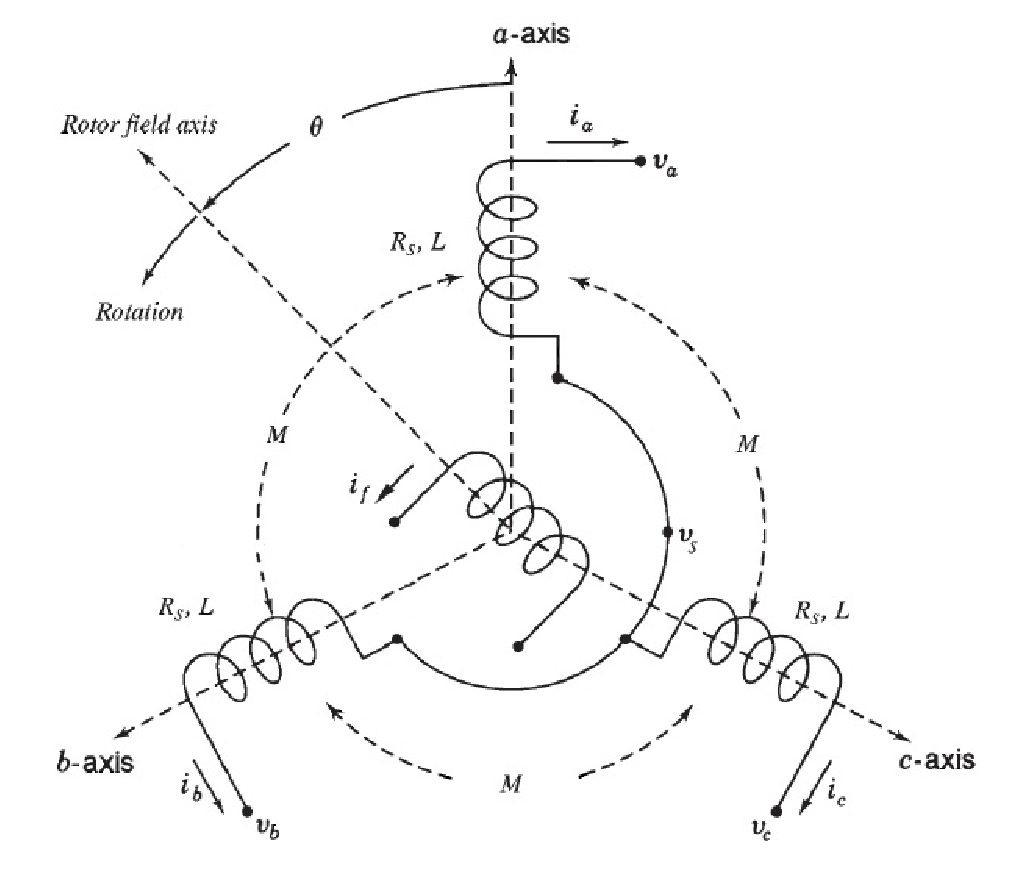
\includegraphics[scale=0.5]{SGStucture}
\par\end{centering} \label{fig:structOfSG}

\caption[Structure of an idealized three-phase round rotor synchronous
generator]{Structure of an idealized three-phase round rotor
synchronous generator, modified from \cite[Figure 3.4]{GrSt2014}.}
\end{figure}
%%%%%%%%%%**********%%%%%%%%%%**********%%%%%%%%%%**********%%%%%%%%%%

The mutual inductance between the rotor coil and each of the stator
coils varies with the rotor angle $\theta$ as follows:
$$ \left[\begin{array}{c} M_{a,f}\\ M_{b,f}\\ M_{c,f}\end{array}
   \right] \m=\m M_{f}\widetilde{\cos}\theta \m,$$
where $M_f>0$ is a constant. The vector of flux linkages of the stator
windings is
$$ \Phi \m=\m \left[\begin{array}{ccc} L & -M & -M\\ -M & L & -M\\
   -M & -M & L \end{array}\right]i + M_f i_f\widetilde{\cos}\theta
   \m.$$
Since there is no neutral line, $i_a+i_b+i_c=0$, so that the previous
equation can be rewritten as 
$$\Phi \m=\m L_s i + M_f i_f \widetilde{\cos}\theta \m,$$
where $L_s=L+M$. We will assume that the rotor current is constant
(or equivalently, the rotor is composed of a permanent magnet). The
stator voltages satisfy
\BEQ{eq:SGTerminalVlotage}
   v - v^n \m=\m -R_{s}i-\frac{\dd\Phi}{\dd t} \m=\m -R_{s}i-L_{s}
   \frac{\dd i}{\dd t} + e \m,
\end{equation}
where $e=\left[e_a\ e_b\ e_c \right] ^\top$ is the back electromotive 
force (EMF) due to the rotor movement (also called synchronous 
internal voltage), given by \vspace{-2mm}
\BEQ{eq:emf}
   e \m=\m M_f i_f\dot{\theta}\widetilde{\sin}\theta \m.
\end{equation}

For a SG with no load, the voltages at each terminal
will be sinusoidal functions. In order to represent the voltages and
currents in a more convenient way, we apply the Park transformation
with respect to the rotor angle:
$$ x_{dq0} \m=\m \left[\begin{array}{c} x_{d}\\ x_{q}\\ x_{0}
   \end{array}\right] \m=\m U(\theta) \left[\begin{array}{c} x_{a}\\
   x_b\\ x_c\end{array}\right] \m=\m U(\theta) x \m,$$
where $x$ is a vector in $abc$ coordinates, $x_{dq0}$
is the same vector in the $dq0$ coordinates, and $U(\theta)$ is the
following unitary matrix:
$$
 U(\theta) \m=\m \sqrt{\frac{3}{2}}\left[\begin{array}{ccc}
   \cos(\theta) & \cos(\theta-\frac{2\pi}{3}) & \cos(\theta-
   \frac{4\pi}{3})\\ -\sin(\theta) & -\sin(\theta-\frac{2\pi}{3})
   & -\sin(\theta-\frac{4\pi}{3})\\ \sqrt{1/2} & \sqrt{1/2} & 
   \sqrt{1/2} \end{array}\right] \m.
$$

Applying the Park transformation to \rfb{eq:SGTerminalVlotage} 
leads to
\BEQ{aPark}
   U(\theta)(v-v^n)-U(\theta)e \m=\m -R_{s}U(\theta)i - L_s 
   U(\theta) \frac{\dd i}{\dd t} \m.
\end{equation}
Now we use that, denoting $i_{dq0}=U(\theta)i$,
$$ \frac{\dd i_{dq0}}{\dd\theta} \m=\m U(\theta)\frac{\dd i}
   {\dd\theta} + \frac{\dd U(\theta)}{\dd\theta}i \m=\m
   U(\theta)\frac{\dd i}{\dd\theta} + \left[\begin{array}{c}
   i_{q}\\ -i_{d}\\ 0 \end{array}\right].$$
This implies that \vspace{-2mm}
$$ \dot{i}_{dq0} \m=\m \frac{\dd i_{dq0}}{\dd\theta} \cdot \frac
   {\dd\theta}{\dd t} \m=\m U(\theta)\dot{i} + \o\left[\begin{array}
   {c} i_q\\ -i_d\\ 0 \end{array}\right] \m,$$
where 
$$\o=\dot{\theta}.$$
 We rewrite \rfb{aPark} as follows:
\BEQ{eq:idiqDynamics}
   L_s\frac{\dd}{\dd t}\nm\left[\nm\begin{array}{c} i_d\\ i_q\\ i_0
   \end{array}\nm\right] - L_s \o \left[\nm\begin{array}{c} i_q\\ -i_d
   \\ 0 \end{array}\nm\right] = -R_s\left[\begin{array}{c} i_d\\
   i_q\\ i_0 \end{array}\right] + \left[\nm \begin{array}{c} e_d-v_d
   \\ e_q-v_q\\ \tilde v\end{array}\nm\right],
\end{equation}
where $\tilde v=e_0-v_0+v^n_0$. Here we have used that (obviously)
$v^n_d=v^n_q=0$. Since there is no neutral connection, $i_0=0$, hence
$\tilde v=0$. Applying the Park transformation to \rfb{eq:emf} gives
$$ \left[\begin{array}{c} e_d\\ e_q \end{array}\right] \m=\m -\sqrt
   {\frac{3}{2}} M_{f} \left[ \begin{array}{c} 0\\ \o i_f
   \end{array}\right] \m.$$
We denote 
$$m=\sqrt{\frac{3}{2}}M_{f}.$$ If we substitute the last
formula into \rfb{eq:idiqDynamics}, we get
\BEQ{eq:idiqDynamicsWithExIf}
   L_s\frac{\dd}{\dd t} \nm \left[\nm \begin{array}{c}
   i_d\\ i_q \end{array} \nm\right] = -R_s\left[\nm \begin{array}{c}
   i_d\\ i_q \end{array} \nm\right]+\o L_s\left[\nm\nm \begin{array}
   {c} i_q\\ -i_d\end{array} \nm\nm\right]\\ -m\left[\nm\nm 
   \begin{array}{c} 0\\ \o i_f\end{array} \nm\nm\right] - \left[\nm 
   \begin{array}{c} v_d\\ v_q \end{array} \nm\right] .
\end{equation}

The rotational dynamics of the rotor is given by
\BEQ{eq:mechanicalPart}
   J\dot{\omega} \m=\m T_{m}-T_{e}-D_{p} \omega \m,
\end{equation}
where $J$ is the moment of inertia of the rotor, $T_m-D_p\o$ is is the
mechanical torque coming from the prime mover, $T_e$ is the
electromagnetic torque developed by the generator, and $D_p$ is a the
frequency droop coefficient employed in the prime movers connected to the generators. If any viscous friction is present, it can be absorbed into the term $D_p\omega$. The feedback term $D_p\o$ is used in
order to control the frequency of the grid, see \cite{Kundur},
\cite{PoDoBu:13}, \cite{CaTa:14}, \cite{ZhWe:11}. $T_e$ can be found
using energy consideration. It is easy to see that the magnetic 
energy stored in the generator is
$$ E_{mag} \m=\m \half \left(\langle i,L_s i \rangle + L_f i_f^2
   \right) + M_f i_f \langle i,\widetilde{\cos}\theta \rangle \m.$$
The electromagnetic torque can be calculated as follows:
$$ T_e \m=\m \frac{\partial E_{mag}}{\partial\theta}|_{\Phi,\Phi_f
   \ const.} \m=\m - \frac{\partial E_{mag}}{\partial\theta}|_{i,
   i_f\ const.}$$
(see \cite{ZhWe:11}), whence
$$ T_e \m=\m M_f i_f \left\langle i,\frac{\dd\tilde{\cos}\theta}
   {\dd\theta} \right\rangle \m=\m M_f i_f \langle i,\widetilde
   {\sin} \theta\rangle \m=\m -m i_f i_q \m.$$
Using \rfb{eq:idiqDynamicsWithExIf}, \rfb{eq:mechanicalPart}
and the last formula, we obtain
\BEQ{eq:SingleSGDynamics}
   \frac{\dd}{\dd t}\nm\left[\nm \begin{array}{c} L_s i_d\\ L_s i_q\\ 
   J\o\end{array} \nm\right] = \left[\nm \begin{array}{ccc} -R_s & 
   \o L_s & 0\\ -\o L_s & -R_s & -mi_f\\ 0 & mi_f & -D_p \end{array}
   \nm\right] \nm \left[\nm \begin{array}{c} i_d\\ i_q\\ \o 
   \end{array} \nm\right] + \left[\nm\nm \begin{array}{c} -v_d\\ -v_q
   \\ T_m \end{array} \nm\nm\right].
\end{equation}
This third order nonlinear dynamical system represents the dynamics
of a single SG with constant field current, if we ignore the dynamics of the rotor 
angle $\theta$. 

\section{TICSG modeling}

In this section we develop the TICSG model that represent a microgid composed of two identical SGs connected in parallel with a resistive load, assuming constant field currents (see Figure \ref{fig:TICSGThreePhase}).

We denote the SG rotor angles by  $\theta_{1}$ and $\theta_{2}$. We assume that identical prime movers act on the generators, producing the torques  $T_{m}-D_p \omega_i$ where $T_m>0$, $D_p>0$ and $i \in \{1,2\}$. By symmetry,
we assume that the voltages at the (non-connected) midpoints of the
generators and the load are zero.

We denoted the phase voltages and currents of the first generator by: $v_{1}=\left[v_{a1}\  v_{b1}\  v_{c1}
\right]^\top$ and $i_{1}=\left[i_{a1}\  i_{b1}\  i_{c1}
\right]^\top$  respectively.
Similarly, we denoted the phase voltages and currents of the second generator as: $v_{2}=\left[v_{a2}\  v_{b2}\  v_{c2}
\right]^\top$ and $i_{2}=\left[i_{a2}\  i_{b2}\  i_{c2}
\right]^\top$ respectively.

We denote by $Z$ the impedance of each SG stator. This impedance is comprised by the resistive impedance of the stator coil $R_s$ and the inductive impedance of the stator, namely $Z\left(s\right)=R_{s} + sL_{s}$. The line that connects the SG to the load has its impedance $Z_l$ that can be modeled  as a resistance and an inductance in series, but these values can simply be added to the parameters $R_s$ and $L_s$ of the SG.
After this simplification, each phase of the circuit from Figure \ref{fig:TICSGThreePhase} is presented at Figure \ref{fig:TICSGOnePhase}.


%%%% Figure Tree phase TICSG system.
\begin{figure}[!htb]
\begin{circuitikz}[american voltages,scale=0.6, transform shape]
\draw   (0,0) node[sground] {}   to [V,v^<=$e_{j1}$] (0,3) {}   to [R=$R_s$,i>=$i_{j1}$] (3,3){}   to [L=$L_s$] (5,3){}   to [R=$R_L$, *-] (5,0){}    to  (5,0) node[sground] {};   
\draw    (4.5, 2.5) to [open,v=$v_L$] (4.5,0);
\draw   (10,0) node[sground] {}   to [V,v^<=$e_{j2}$] (10,3) {}   to [R=$R_s$,i>=$i_{j2}$,mirror] (7,3){}   to [L=$L_s$, mirror] (5,3){};  
 \node[draw] at (-1,4) {$j \in \{a,b,c\}$}; \end{circuitikz} 

\caption{ A microgrid comprising two identical SGs and a resistive load - equivalent circuit diagram for one phase, $j \in \{a,b,c\}.$}

\label{fig:TICSGOnePhase}
\end{figure}

%%%%%%%%%

In order to use the fourth order model of a single SG \eqref{eq:SingleSGDynamics} in the two SGs system, we apply  the Park transformation, on each SG  terminal voltages: $\left[ v_{di}\ v_{qi}\  v_{0i} \right]^\top=U(\theta_{i})\left[v_{ai}\ v_{bi}\ v_{ci}  \right]^\top$,  and currents $\left[v_{di}\ v_{qi}\  v_{0i} \right]^\top=U(\theta_{i})\left[v_{ai}\ v_{bi}\ v_{ci}  \right]^\top$,  ($i \in \{1,2\}$).

An expression of the voltage at each SG terminal is:
$$v_1=v_2=v_L=R_{L}(i_{1}+i_{2})$$

Rewriting this equation for the first SG after applying the Park transformation yields:

$$
\left[\begin{array}{c}
v_{d1}\\
v_{q1}\\
v_{01}
\end{array}\right]=R_{L}\left[\begin{array}{c}
i_{d1}\\
i_{q1}\\
i_{01}
\end{array}\right]+R_{L}U(\theta_{1})\left[\begin{array}{c}
i_{a2}\\
i_{b2}\\
i_{c2}
\end{array}\right]
$$

Because Park transformations argument is  $\theta_1$,  the second SG current can't be transformed directly to the d-q coordinates:   $U(\theta_{1})\left[ i_{a2}\ i_{b2}\ i_{c2}\right]^\top \neq \left[ i_{d2}\ i_{q2}\ i_{02}\right]$. 

We express  the currents of the second SG in the d-q coordinates by using the inverse Park transformation: 
\BEQ{eq:TICSGVolAndCurr}
 \left[\begin{array}{c}
v_{d1}\\
v_{q1}\\
v_{01}
\end{array}\right]=R_{L}\left[\begin{array}{c}
i_{d1}\\
i_{q1}\\
i_{01}
\end{array}\right]+R_{L}U(\theta_{1})U(\theta_{2})^{-1}\left[\begin{array}{c}
i_{d2}\\
i_{q2}\\
i_{02}
\end{array}\right].
\end{equation}

We denote $$\delta=\theta_{2}-\theta_{1}.$$

A simple computation shows that 
\BEQ{eq:ParkChangeAngle}
  U(\theta_{1})U(\theta_{2})^{-1}=\left[\begin{array}{ccc}
\cos(\delta) & -\sin(\delta) & 0\\
\sin(\delta) & \cos(\delta) & 0\\
0 & 0 & 1
\end{array}\right].
\end{equation}

Since the SGs don't have a neutral connection,  by using Kirchhoff's laws we obtain that $i_{01}=i_{02}=0$.  Substituting this into \eqref{eq:TICSGVolAndCurr} and \eqref{eq:ParkChangeAngle} shows that $v_{01} = 0$.

Substitute \eqref{eq:SingleSGDynamics} and \eqref{eq:ParkChangeAngle} into \eqref{eq:TICSGVolAndCurr}  gives:

\[
\varLambda\dot{z}_{1}=\mathcal{A}(\omega_{1})z_{1}+T_{m}e_{3}-\mathcal{B}(\delta)z_{2}
\]
where we have denoted
 $$z_{i}=\left[i_{di}\ i_{qi}\  \omega_{i}\right]^\top,\quad i\in\{1,2\},$$

\[
\varLambda=\left[\begin{array}{ccc}
L_{s} & 0 & 0\\
0 & L_{s} & 0\\
0 & 0 & J
\end{array}\right],
\]

\[
\mathcal{A}(\omega)=\left[\begin{array}{ccc}
-R_{tot} & \omega L_{s} & 0\\
-\omega L_{s} & -R_{tot} & -mi_{f}\\
0 & mi_{f} & -D_{p}
\end{array}\right],
\]
\[\mathcal{B}(\delta)=\left[\begin{array}{ccc}
R_{L}\cos(\delta) & -R_{L}\sin(\delta) & 0\\
R_{L}\sin(\delta) & R_{L}\cos(\delta) & 0\\
0 & 0 & 0
\end{array}\right],
\]
$$e_{3}=\left[0\ 0\ 1\right]^\top, \quad  R_{tot}=R_{s}+R_{L}.$$

Of course a symmetric equation holds for the second generator:

\[
\varLambda\dot{z}_{2}=\mathcal{A}(\omega_{2})z_{2}+T_{m}e_{3}-\mathcal{B}(-\delta)z_{1}
\]

We denote the angular velocities  of the SG rotors by $\omega_i = \dot{\theta_i}$ where $i \in \{1,2\}$. 
An additional ODE for $\delta$ is:

\[
\dot{\delta}=\omega_{2}-\omega_{1}.
\]

Rewriting the entire system dynamics gives:

\begin{equation}
\begin{array}{ccc}
\frac{d}{dt}\left[\begin{array}{c}
\varLambda z_{1}\\
\varLambda z_{2}\\
\delta
\end{array}\right] & = & \left[\begin{array}{c|c|c}
\mathcal{A}(\omega_{1}) & -\mathcal{B}(\delta) & 0\\
\hline -\mathcal{B}(-\delta) & \mathcal{A}(\omega_{2}) & 0\\
\hline -e_{3}^{T} & e_{3}^{T} & 0
\end{array}\right]\left[\begin{array}{c}
z_{1}\\
z_{2}\\
\delta
\end{array}\right]\\
 &  & +T_{m}\left[\begin{array}{c}
e_{3}\\
e_{3}\\
0
\end{array}\right]
\end{array}\label{eq:TICSGDynamics}
\end{equation}

We refer this seventh order nonlinear dynamic system as the TICSG model.


\begin{lemma}\label{lemma:forewordComplete}
The TICSG system is foreword complete, i.e. for any initial state $\left[ z_1^{0\top} \ z_2^{0\top}  \ \delta^{0}  \right]^\top \in \mathbb{R}^7 $, the (unique) solution of the TICSG system is defined for all $t>0$.
\end{lemma}
\begin{proof}
(This proof is in the spirit of \cite[p.7]{NaWe:15}).

The right hand side of the TICSG model \eqref{eq:TICSGDynamics} is a locally Lipschitz function on its state space. For any initial state it follows from standard well posedness results (see for instance \cite[Ch. 3]{Khalil}) that there exists a unique solution $( z_1 \ z_2  \ \delta  )$ for \eqref{eq:TICSGDynamics} defined on a maximal time interval $[0,T_{max})$, with $T_{max} > 0$. We will show via contradiction that $T_{max}=\infty$. Suppose that $T_{max}$  is finite. For each $t\in [0,T_m)$ define 
$$V\left(\left[\begin{array}{c}
z_1\\ z_2
\end{array}\right]\right) =  \left[z_1^\top\ z_2^\top\right]\left[\begin{array}{cc}
\varLambda & 0\\ 0 & \varLambda
\end{array}\right]\left[\begin{array}{c}
z_1\\ z_2
\end{array}\right].$$
Then 
$$\dot{V}(t) = 2\left[z_1^\top\ z_2^\top\right]\left[\begin{array}{cc}
\varLambda & 0\\ 0 & \varLambda
\end{array}\right]\left[\begin{array}{c}
\dot{z_1}\\ \dot{z_2}
\end{array}\right].$$ 
After substitute \eqref{eq:TICSGDynamics} we get
$$
\begin{aligned}
{V}(t) &= 2\left[z_1^\top\ z_2^\top\right]\left[\begin{array}{cc}
\varLambda & 0\\ 0 & \varLambda
\end{array}\right] \\ & \left[\begin{array}{c}
\varLambda^{-1}\left(\mathcal{A}(\omega_1)z_1- \mathcal{B}(\delta)z_2+T_me_3\right)
\\ 
\varLambda^{-1}\left(- \mathcal{B}(-\delta)z_1+\mathcal{A}(\omega_2)z_2+T_me_3\right)
\end{array}\right].
\end{aligned}
$$ 
Because $\mathcal{B}(-\delta) = \mathcal{B}^\top(\delta)$ then 
$$
\begin{aligned}
\dot{V}(t) =& 2\left(z_1^\top\mathcal{A}(\omega_1)z_1+z_2^\top\mathcal{A}(\omega_2)z_2\right) \\ +&2\left(-2z_1^\top\mathcal{B}(\delta)z_2 + T_mz_1^\top e_3+ T_mz_2^\top e_3\right)
\end{aligned}
$$ 
explicitly,
$$
\begin{aligned}
\dot{V}(t) &= 2\left(-R_{tot}\left(i_{d1}^2+i_{q1}^2+i_{d2}^2+i_{q2}^2 \right) -D_p\left( \omega_1^2+\omega_2^2\right)\right) \\
& +4R_L\left( -\cos(\delta)i_{d1}i_{d2}-\cos(\delta)i_{q1}i_{q2}-\sin(\delta)i_{q1}i_{d2}\right)\\ &+4 R_L\left(\sin(\delta)i_{q2}i_{d1}\right)
 +2T_m(\omega_1+\omega2).
\end{aligned}
$$ 
This equation can be described in a matrix form

$$
\begin{aligned}
\dot{V(t)} &= -2D_p\left( \omega_1^2+\omega_2^2\right) +2T_m(\omega_1+\omega2)-2\vec{i}^\top A\vec{i}
\end{aligned}
$$ 
where $\vec{i}=[i_{d1}\ i_{q1}\ i_{d2}\ i_{q2}]^\top$ and 
$$
\begin{aligned}
A&=\left[\begin{array}{cc|cc}
R_{tot} & 0 & R_L \cos(\delta) & -R_L \sin(\delta) \\ 
0 & R_{tot} & R_L R_L \sin(\delta) & R_L\cos(\delta) \\ 
\hline
R_L\cos(\delta) & R_L \sin(\delta) & R_{tot} & 0 \\ 
-R_L \sin(\delta) & R_L\cos(\delta) & 0 & R_{tot} 
\end{array}\right]\\&=\left[
\begin{array}{c|c}
A_1 & B \\
\hline
B^* & A_1
\end{array}
\right].
\end{aligned}$$

According to Schur complement condition for positive definiteness, a symmetric matrix $X = \left[
\begin{array}{c|c}
M & N \\
\hline
N^* & Y
\end{array}
\right]$  is positive definite if and only if $M$ and  $\Delta=Y-N^*M^{-1}N$ are both positive definite. it means that in order to show that $A$ is a positive definite we need to show that both $A_1$ and  $A_1-B^*A_1^{-1}B$ are positive definite. $A_1$ is clearly positive definite (it is diagonal matrix with navigate value on the main diagonal). 
$$
A_1-B^*A_1^-1B= \left[\begin{array}{cc}
R_{tot}-\frac{R_L^2}{R_{tot}} & 0  \\ 
0 & R_{tot}-\frac{R_L^2}{R_{tot}}  
\end{array}\right].$$
Because the term $R_{tot}$ is bigger then $R_L$ then $A_1-B^*A_1^-1B$ is positive definite matrix, which implies that A is a positive definite matrix.
Which shows that if either $|i_{d1}|$, $|i_{q1}|$, $|\omega_{1}|$, $|i_{d2}|$, $|i_{q2}|$ or $|\omega_{2}|$ is sufficiently large, then $\dot{V}(t)<0$. Therefore $V$ (and hence $i_{d1}$, $i_{q1}$, $\omega_{1}$, $i_{d2}$, $i_{q2}$ and $\omega_{2}$ are bounded on $[0,T_{max})$ Since $T_{max}$ is bounded then $\delta$ must also be bounded. Hence $(i_{d1},i_{q1},\omega_1,i_{d2},i_{q2},\omega_2)$ are bounded functions on $[0,T_{max})$ which contradict \cite[ Corollary II.3]{JayWeissBS:09}. Therefore  $T_{max} = \infty$.
\end{proof}

%%%%%%%%%%**********%%%%%%%%%%**********%%%%%%%%%%**********%%%%%%%%%%

\section{Analysis of the equilibrium points of the TICSG model \label{sec:equivalence_pont}}

In this section, we study the equilibrium points of the TICSG system. First, we show that  if there exist equilibrium points, they must located on the synchronization subspace or on the anti-synchronization subspace i.e. any equilibrium point $\left[z_1^e \ z_2^e \ \delta^e \right]^\top$ must satisfy $z_1^e=z_2^e$ and $\delta^e=0$ or $\delta^e = \pi$   (modulo $2\pi$). Second, we show that the TICSG system has at least one equilibrium point on the synchronization subspace (i.e with $\delta^e=0$).

\subsection{An equilibrium point must satisfy synchronization condition.}
We  start by investigate the solution of the algebraic equation:  

\begin{equation}
\left[\begin{array}{c|c|c}
\mathcal{A}(\omega_{1}^{e}) & -\mathcal{B}(\delta^{e}) & 0\\
\hline -\mathcal{B}(-\delta^{e}) & \mathcal{A}(\omega_{2}^{e}) & 0\\
\hline -e_{3}^{T} & e_{3}^{T} & 0
\end{array}\right]\left[\begin{array}{c}
z_{1}^{e}\\
z_{2}^{e}\\
\delta^{e}
\end{array}\right]+T_{m}\left[\begin{array}{c}
e_{3}\\
e_{3}\\
0
\end{array}\right]=0
\label{eq:algebricEquation}
\end{equation}

It easy to see that according to the seventh line $$\omega_{1}^{e}=\omega_{2}^{e}=\omega^{e}$$.

From the third and the sixth lines we have: 

$$
\left\{ \begin{array}{c}
mi_{f}i_{q1}^{e}-D_{p}\omega_{1}^{e}+T_{m}=0\\
mi_{f}i_{q2}^{e}-D_{p}\omega_{2}^{e}+T_{m}=0
\end{array}\right.\longrightarrow i_{q1}^{e}=i_{q2}^{e}=i_{q}^{e}
$$

From the first, second, fourth and fifth lines:

$$
 \begin{array}{c}
-R_{tot}i_{d1}^{e}+\omega^{e}L_{s}i_{q}^{e}-R_{L}\cos\delta^{e}i_{d2}^{e}+R_{L}\sin\delta^{e}i_{q}^{e}=0\\
-\omega^{e}L_{s}i_{d1}^{e}-R_{tot}i_{q}^{e}-mi_{f}\omega^{e}-R_{L}\sin\delta^{e}i_{d2}^{e}-R_{L}\cos\delta^{e}i_{q}^{e}=0\\
-R_{tot}i_{d2}^{e}+\omega^{e}L_{s}i_{q}^{e}-R_{L}\cos\delta^{e}i_{d1}^{e}-R_{L}\sin\delta^{e}i_{q}^{e}=0\\
-\omega^{e}L_{s}i_{d2}^{e}-R_{tot}i_{q}^{e}-mi_{f}\omega^{e}+R_{L}\sin\delta^{e}i_{d1}^{e}-R_{L}\cos\delta^{e}i_{q}^{e}=0
\end{array}
$$
By denoting:
\[
M=\left[\begin{array}{cc}
-R_{tot} & -R_{L}\cos\delta^{e}\\
-\omega^{e}L_{s} & -R_{L}\sin\delta^{e}\\
-R_{L}\cos\delta^{e} & -R_{tot}\\
R_{L}\sin\delta^{e} & -\omega^{e}L_{s}
\end{array}\right]
\]

and 

\[
n=\left[\begin{array}{c}
i_{q}^{e}\left(\omega^{e}L_{s}+R_{L}\sin\delta^{e}\right)\\
-mi_{f}\omega^{e}-i_{q}^{e}\left(R_{tot}+R_{L}\cos\delta^{e}\right)\\
i_{q}^{e}\left(\omega^{e}L_{s}-R_{L}\sin\delta^{e}\right)\\
-mi_{f}\omega^{e}-i_{q}^{e}\left(R_{tot}+R_{L}\cos\delta^{e}\right)
\end{array}\right]
\]
we rewrite these lines in the following way:

\begin{equation}
M\left[\begin{array}{c}
i_{d1}^{e}\\
i_{d2}^{e}
\end{array}\right]=n.\label{eq:equilibrium_system}
\end{equation}

Now, we  show by contradiction that any equilibrium point must satisfy: $\sin\delta^e=0$.
We use the Rouch\'e Capelli theorem:  Any liner equations system with the form  $Mx=n$ has a  solution if and only if rank$\left[M|n\right]=$rank$\left[M\right].$

If we negated to assume that $\sin\delta^{e}\ne0$, then a simple calculation shows that under this assumption  rank$\left[M|n\right]=3$ must hold.

Obviously, rank$\left[M\right]\le2$.  The Rouch\'e Capelli theorem implies that under the
previous assumption the linear equations system \eqref{eq:equilibrium_system} does not have any solution. It proves that  if the TICSG system has an equilibrium point, it must satisfied: $\sin\delta^{e}=0$ means that : $\delta^{e}=0$ or $\delta^e = \pi$ (modulo $2\pi$).

After subtitling $\sin\delta^{e}=0$
and $\cos\delta^{e}=\pm 1$, the linear equations system  \eqref{eq:equilibrium_system} becomes:

$$
M=\left[\begin{array}{cc}
-R_{tot} & \mp R_{L}\\
-\omega^{e}L_{s} & 0\\
  \mp R_{L} & -R_{tot}\\
0 & -\omega^{e}L_{s}
\end{array}\right]
$$

and 

$$
n=\left[\begin{array}{c}
i_{q}^{e}\omega^{e}L_{s}\\
-mi_{f}\omega^{e}-i_{q}^{e}\left(R_{tot} \pm R_{L}\right)\\
i_{q}^{e}\omega^{e}L_{s}\\
-mi_{f}\omega^{e}-i_{q}^{e}\left(R_{tot} \pm R_{L}\right)
\end{array}\right]
$$

This solution of this system is: $i_{d1}^{e}=i_{d2}^{e}$.



\subsection{The TICSG system has at least one equilibrium point on the synchronization subspace}
Here, we show that the TICSG system has at least one equilibrium point on the three dimensional subspace
\begin{equation}
\mathscr{E}=\{ \left[z_1 \ z_2 \ \delta  \right]^\top   |   z_1=z_2,\delta= 0\}\label{eq:SyncSubspace}
\end{equation}
Which we call the \textit{synchronization subspace}.

After substituting condition \eqref{eq:SyncSubspace} into \eqref{eq:algebricEquation} ,we get:

\begin{equation}
\left[\begin{array}{ccc}
-R_{s}-2R_{L} & \omega^{e}L_{s} & 0\\
-\omega^{e}L_{s} & -R_{s}-2R_{L} & -mi_{f}\\
0 & mi_{f} & -D_{p}
\end{array}\right]\left[\begin{array}{c}
i_{d}^{e}\\
i_{q}^{e}\\
\omega^{e}
\end{array}\right]=\left[\begin{array}{c}
0\\
0\\
-T_{m}
\end{array}\right]\label{eq:equilbrium_algebric_eq}
\end{equation}

We take scalar products on both sides with $z^{e}$:

\[
\left(R_{tot}+R_{L}\right)\left((i_{d}^{e})^{2}+(i_{q}^{e})^{2}\right)=\left(T_{m}-D_{p}\omega^{e}\right)\omega^{e}
\]

This equation makes perfect physical sense. Indeed, assume that there
is no actual friction in the machine, $D_{p}$ is created by feedback,
so that $T_{m}-D_{p}\omega^{e}$ is the mechanical torque applied
to one generator, and then $\left(T_{m}-D_{p}\omega^{e}\right)\omega^{e}$
is the mechanical power entering one generator. On the other hand,
it is easy to see that $\left(R_{tot}+R_{L}\right)\left((i_{d}^{e})^{2}+(i_{q}^{e})^{2}\right)=\left(R_{s}+2R_{L}\right)\left(i_{a}^{2}+i_{b}^{2}+i_{c}^{2}\right)$
which is exactly half of the power dissipated in all the resistors,
hence it is the electric power leaving one generator.

From \eqref{eq:equilbrium_algebric_eq} we derive a scalar
equation to determine the equilibrium velocity $\omega^{e}$.
From the last line of the matrix equation\eqref{eq:equilbrium_algebric_eq} we have

\begin{equation}
T_{m}-D_{p}\omega^{e}=-mi_{f}i_{q}^{e}\label{eq:eq_0_first_eq}
\end{equation}

The left side of this equation is the mechanical torque acting on each
generator at equilibrium.

The first line of  \eqref{eq:equilbrium_algebric_eq}
is $-\left(R_{tot}+R_{L}\right)i_{d}^{e}+\omega^{e}L_{tot}i_{q}^{e}=0$,
\quad hence

\[
i_{d}^{e}=\frac{\omega^{e}L_{s}}{R_{tot}+R_{L}}i_{q}^{e}.
\]

From \eqref{eq:eq_0_first_eq} 
\begin{equation}
i_{q}^{e}=\frac{T_{m}-D_{p}\omega^{e}}{-mi_{f}}\label{eq:iq_0_}
\end{equation}

Combining the last two formulas,

\begin{equation}
i_{d}^{e}=-\frac{\omega^{e}L_{s}}{R_{tot}+R_{L}}\frac{T_{m}-D_{p}\omega^{e}}{mi_{f}}\label{eq:id_0_}
\end{equation}

The second line of the matrix equation on \eqref{eq:eq_0_first_eq}
is 
$$\omega^{e}L_{s}i_{d}^{e}+\left(R_{tot}+R_{L}\right)i_{q}^{e}+mi_{f}\omega^{e}=0.$$
Substituting in this equation the expressions for $i_{q}^{e}$ and $i_{d}^{e}$ yields the following cubic equation in $\omega^e$, where we denote $R_T = R_L+R_{tot}$:

\begin{equation}
\begin{split}
D_{p}L_{s}^{2}\left(\omega^{e}\right)^{3}-T_{m}L_{s}^{2}\left(\omega^{e}\right)^{2} +\left(D_{p}R_T^{2}+m^{2}i_{f}^{2}R_T\right) \omega^{e} \\ -T_{m}R_T^{2}=0
\end{split}\label{eq:cuibi_eq}
\end{equation}

Let us denote the polynomial of order 3 in \eqref{eq:cuibi_eq} by
$p(\omega^{e})$. 
Clearly
$$p(0)=-T_{m}R_T^{2}<0.$$
On the other hand, we note that 
$$
p(\frac{T_{m}}{D_{p}}) =m^{2}i_{f}^{2}R_T\frac{T_{m}}{D_{p}}>0.
$$

Hence, \eqref{eq:cuibi_eq} has at least one solution in the interval
$\omega^{e}\in\left(0,\frac{T_{m}}{D_{p}}\right)$.

This shows that the TICSG system has at least one equilibrium point  that located on the synchronization subspace \eqref{eq:SyncSubspace}.

Note, that the anti-synchronization manifold  $\mathscr{E} '=\{ \left[z \ z \ \delta  \right]^\top   |  \delta=\pi \}$ may also have equilibrium points.
%%%%%%%%%%**********%%%%%%%%%%**********%%%%%%%%%%**********%%%%%%%%%%

\section{Synchronization}

In this section, we show that the synchronization subspace $\mathscr{E}$ from \eqref{eq:SyncSubspace}, is invariant and locally exponentially stable for the TICSG model \eqref{eq:TICSGDynamics}.
We start by rewriting the TICSG model in new coordinates. Then, we  prove that under
some conditions, the TICSG is globally exponentially
stable in the subspce  $\mathscr{E}$. Finally, we use the main result from  \cite{AndrieuJayawardhanaPraly},
to show the stability of the system near the synchronization subspace.

\section{Modeling the synchronization problem:}\label{sec:SyncProbModel}
The TICSG system has the following structure:
$$ \tilde{\Lambda}\frac{d}{dt}\left[z_1\ z_2\ \delta\right]^{\top}= f\left( \left[z_1\ z_2\ \delta\right]^{\top} \right)$$
where $\tilde{\Lambda} = diag \left( \Lambda,\Lambda,1 \right) $.
In order to show synchronization, it is convenient to introduce new state variables $e \in \mathbb{R}^4$ and $x \in \mathbb{R}^3$ by
$$e =  \left[ \begin{array}{c}
z_2 - z_1\\
\delta
\end{array} \right] = \left[e_d\ e_q\ e_{\omega}\ \delta \right]^\top $$
and 
$$x =z_1+z_2 = \left[ x_d\ x_q\ x_\omega\right]^\top.$$  

Then the TICSG model \eqref{eq:TICSGDynamics} can be rewritten as

\begin{equation}
\dot{e}=F(e,x) , \quad \dot{x}=G(e,x),\label{eq:sync_sestem}
\end{equation}
for some functions $F$ and $G$.  From \eqref{eq:TICSGDynamics}:
$$
\begin{aligned}
\Lambda(\dot{z}_{2}-\dot{z}_{1})&=\mathcal{A}(\omega_{2})z_{2}+T_{m}e_{3}-\mathcal{B}(-\delta)z_{1}\\&-\left(\mathcal{A}(\omega_{1})z_{1}+T_{m}e_{3}-\mathcal{B}(\delta)z_{2}\right)
\end{aligned}
$$
Calculating  $F$:
$$
\begin{aligned}
&  \left[\begin{array}{cc}
\varLambda & 0\\
0 & 1
\end{array}\right] \frac{d}{dt}\left[\begin{array}{c}
e_{d}\\
e_{q}\\
e_{\omega}\\
\delta
\end{array}\right]  =  \\ & \left[\begin{array}{c}
-R_{tot}(i_{d2}-i_{d1})+L_{s}(\omega_{2}i_{q2}-\omega_{1}i_{q1})\\
-L_{s}(\omega_{2}i_{d2}-\omega_{1}i_{d1})-R_{tot}(i_{q2}-i_{q1})-mi_{f}(\omega_{2}-\omega_{1})\\
mi_{f}(i_{q2}-i_{q1})-D_{p}(\omega_{2}-\omega_{1})\\
-(\omega_{2}-\omega_{1})
\end{array}\right]\\
 + & \left[\begin{array}{c}
R_{L}\cos(\delta)(i_{d2}-i_{d1})-R_{L}\sin(\delta)(i_{q2}+i_{q1})\\
R_{L}\cos(\delta)(i_{q2}-i_{q1})+R_{L}\sin(\delta)(i_{d2}+i_{d1})\\
0\\
0
\end{array}\right].
\end{aligned}
$$

Because the following equation   
$$(a+b)(x-y)+(a-b)(x+y)=2(ax-by)$$
holds for any $x$, $y$, $a$ and $b$, it implies that:
$$
\begin{aligned}
\omega_{2}i_{q2}-\omega_{1}i_{q1}= &\frac{1}{2}\left[(\omega_{1}+\omega_{1})(i_{q2}-i_{q1})+(\omega_{2}-\omega_{1})(i_{q2}+i_{q1})\right] \\ =&\frac{x_{w}e_{q}+e_{w}x_{q}}{2}
\end{aligned}
$$
 
and the previous equation can be rewritten as:
$$
\dot{e}  = F(e,x) =\left[\begin{array}{cc}
\varLambda & 0\\
0 & 1
\end{array}\right]^{-1}\left(A_e\left(x,e\right) e +B_e\left(x,e\right)  \right)
$$
Where 

$$
\begin{aligned}
&A_e\left(x,e\right)  = \\ & \left[\begin{array}{cccc}
-R_{tot}+R_{L}\cos\delta & \frac{L_{s}}{2}x_{\omega} & \frac{L_{s}}{2}x_{q} & 0\\
-\frac{L_{s}}{2}x_{\omega} & -R_{tot}+R_{L}\cos\delta & -\frac{L_{s}}{2}x_{d}-mi_f & 0\\
0 & mi_{f} & -D_{p} & 0\\
0 & 0 & 1 & 0
\end{array}\right]
\end{aligned}
$$ 
and
$$
B_e\left(x,e\right) = 
\left[\begin{array}{c}
-R_{L}\sin(\delta)x_{q}\\
R_{L}\sin(\delta)x_{d}\\
0\\
0
\end{array}\right].
$$

Note that the synchronization subspace $\mathscr{E}$ from \eqref{eq:SyncSubspace}, in the new coordinates, becomes $\mathscr{E}=\left\{\left[ \begin{array}{c}
x \\
e
\end{array}\right] \in\mathbb{R}^{7}|e=0 \right\}$.
We note that $F(0,x)=0$, which shows that 
$\mathscr{E} $ is invariant.

For the $x$ dynamics we have:

$$
\begin{aligned}
\Lambda\dot{x}= & \mathcal{A}(\omega_{1})z_{1}+T_{m}e_{3}-\mathcal{B}(\delta)z_{2}\\+&\mathcal{A}(\omega_{2})z_{2}  +T_{m}e_{3}-\mathcal{B}(-\delta)z_{1}.
\end{aligned}
$$

$$
\begin{aligned}
&\Lambda\frac{d}{dt}\left[\begin{array}{c}
x_{d}\\
x_{q}\\
x_{\omega}
\end{array}\right]  = \\
 & \left[\begin{array}{c}
-R_{tot}(i_{d1}+i_{d2})+L_{s}(\omega_{1}i_{q1}+\omega_{2}i_{q2})\\
-L_{s}(\omega_{1}i_{d1}+\omega_{2}i_{d2})-R_{tot}(i_{q1}+i_{q2})-mi_{f}(\omega_{1}+\omega_{2})\\
mi_{f}(i_{q1}+i_{q2})-D_{p}(\omega_{1}+\omega_{2})+2T_{m}
\end{array}\right]\\
 +& \left[\begin{array}{c}
-R_{L}\cos(\delta)(i_{d1}+i_{d2})-R_{L}\sin(\delta)(i_{q1}-i_{q2})\\
-R_{L}\cos(\delta)(i_{q1}+i_{q2})+R_{L}\sin(\delta)(i_{d1}-i_{d2})\\
0
\end{array}\right]
\end{aligned}
$$

Since the identity 
$$
(a+b)(x+y)+(a-b)(x-y)=2(ax+by)
$$
holds for any $x$, $y$, $a$ and $b$, it follows that
$$
\begin{aligned}
\omega_{1}i_{q1}+\omega_{2}i_{q2} &=\frac{1}{2}\left[(\omega_{1}+\omega_{2})(i_{q1}+i_{q2})+(\omega_{1}-\omega_{2})(i_{q1}-i_{q2})\right]\\ & =\frac{x_{w}x_{q}+e_{w}e_{q}}{2}
\end{aligned}
$$

and similarly

$$
\omega_{1}i_{d1}-\omega_{2}i_{d2}=\frac{x_{w}x_{d}+e_{w}e_{d}}{2}
$$ 

The $x$ dynamics can be rewritten as:
$$ \dot{x}=G \left( x,e\right)= \Lambda^{-1}\left(A_x \left(x,e \right) x + B_x \left( x,e\right) \right), $$
where
$$
A_x \left(x,e \right)=\left[\begin{array}{ccc}
-R_{tot}-R_{L}\cos(\delta) & \frac{L_{s}}{2}x_{\omega} & 0\\
-\frac{L_{s}}{2}x_{\omega} & -R_{tot}-R_{L}\cos(\delta) & -mi_f\\
0 & mi_{f} & -D_{p}
\end{array}\right]
$$

$$
B_x \left(x,e \right)=\left[\begin{array}{c}
\frac{L_{s}}{2}e_{\omega}e_{q}-R_{L}\sin(\delta)e_{q}\\
-\frac{L_{s}}{2}e_{\omega}e_{d}-R_{L}\sin(\delta)e_{d}\\
2T_{m}
\end{array}\right]
$$

\subsection{Globally exponentially stability of the TICSG system on the synchronization subspace }

In this subsection, we provide sufficient conditions for the equilibrium
point which located on the synchronization subspace $\mathscr{E}=\left\{ \left[ e\ x \right]^\top \in\mathbb{R}^{7}|e=0\right\} $,  to be a globally exponential stable equilibrium point, for trajectories with initial condition that lies on the $\mathscr{E}$ subspace.  Because we showed that  $\mathscr{E}$ is invariant subspace, it means that any trajectory that starts within this subspace, remains inside it.

We denote the state variables of of these trajectories as $\tilde{x} = \left[x_d \ x_q\ x_\omega \right]^\top$. 

The dynamics of these trajectories is (denoted as $\tilde{G}$):
$$
\dot{\tilde{x}}=\tilde{G}(\tilde{x})=G(0,\tilde{x})=
 \Lambda^{-1} A\left( \tilde{x}_\omega \right) \tilde{x}+\Lambda^{-1} B 
$$

Where we denote:
$$
A\left( \tilde{x}_\omega \right)=A_x\left(0, \tilde{x}_\omega \right) =  
 \left[\begin{array}{ccc}
-R_T & \frac{L_{s}}{2}\tilde{x}_{\omega} & 0\\
-\frac{L_{s}}{2}\tilde{x}_{\omega} & -R_T & -mi_f\\
0 & mi_{f} & -D_{p}
\end{array}\right]
$$
and
$$
B = B_x\left(0, \tilde{x}_\omega \right)  =  
 \left[\begin{array}{c}
0\\
0\\
2T_{m}
\end{array}\right].
$$

This system describes the two SGs with perfect synchronization between each other.

Because the TICSG system has at list one equilibrium point on the $\mathscr{E}$ subspace, it means that $\tilde{G}(\tilde{x})$ has at list one equilibrium point 
$\tilde{x}^{e}=\left[\tilde{x}_{d}^{e}\ \tilde{x}_{q}^{e}\ \tilde{x}_{\omega}^{e} \right]^\top = 2z^e$ (recall that by definition $x = z_1 + z_2$).

\begin{equation}
\tilde{G}(\tilde{x}^{e})=0\rightarrow\varLambda^{-1}A(\tilde{x}_{\omega}^{e})\tilde{x}^{e}+\varLambda^{-1}\left[\begin{array}{c}
0\\
0\\
2T_{m}
\end{array}\right]=0\label{eq:G_at_equilibrium}
\end{equation}

In order to shift the equilibrium point into the origin, we introduce the new  coordinates
$$
\hat{x}\coloneqq\tilde{x}-\tilde{x}^{e}
$$

A natural Lyapunov function candidate for this system is 
$$
V(\hat{x})\coloneqq\frac{1}{2}L_{s}\left(\hat{x}_{d}^{2}+\hat{x}_{q}^{2}\right)+\frac{1}{2}J\tilde{\omega}^{2}=\frac{1}{2}\hat{x}^{T}\varLambda\hat{x}.
$$

It is easy to see that:
$$
\frac{1}{2} min\left\{L_{s},J\right\}|\hat{x}|{}^{2}\leq V(\hat{x})\leq \frac{1}{2} max\left\{L_{s},J\right\}|\hat{x}|{}^{2}
$$

$$
\left|\frac{\partial V}{\partial\hat{x}}\right|=\left|\varLambda\hat{x}\right|\leq max\left\{L_{s},J\right\}\left|\hat{x}\right|
$$

We calculate $\dot{V}(\hat{x})$ in order to show that under some
conditions, $\dot{V}(\hat{x})\leq\alpha|\hat{x}|{}^{2}$, for some
$\alpha.$ This  proves that $\tilde{G}(\tilde{x})$ is globally
exponentially stable (see for instance theorum 5.17, p195 at \cite{Sastry}).

$$
\dot{V}(\hat{x})=\left(\frac{\partial V}{\partial\hat{x}}\right)^{T}\dot{\hat{x}}
$$

\begin{equation}
\dot{\hat{x}}=\dot{\tilde{x}}=\varLambda^{-1}A(\tilde{x}_\omega)\tilde{x}+\varLambda^{-1}\left[\begin{array}{c}
0\\
0\\
2T_{m}
\end{array}\right]\label{eq:x_hat_dynamic}
\end{equation}
 
We rewrite  $A(\tilde{x}_{\omega})$ as a sum of a constant symmetric
matrix, constant skew symmetric matrix and a skew symmetric matrix
which depends on $\hat{x}_{\omega}$:
$$ 
A(\tilde{x}_{\omega})\tilde{x}=\left[R+J(\tilde{x}_{\omega}^{e})+\Delta(\hat{x}_{\omega})\right](\hat{x}+\tilde{x}^{e})
$$
While
$$
R\coloneqq\left[\begin{array}{ccc}
-R_T & 0 & 0\\
0 & -R_T & 0\\
0 & 0 & -D_{p}
\end{array}\right]
$$

$$
J\coloneqq\left[\begin{array}{ccc}
0 & \frac{L_{s}}{2}\tilde{\omega}^{e} & 0\\
-\frac{L_{s}}{2}\tilde{\omega}^{e} & 0 & -mi_f\\
0 & mi_{f} & 0
\end{array}\right]
$$

$$
\Delta(\hat{x}_{\omega})\coloneqq\left[\begin{array}{ccc}
0 & \frac{L_{s}}{2}\hat{x}_{\omega} & 0\\
-\frac{L_{s}}{2}\hat{x}_{\omega} & 0 & 0\\
0 & 0 & 0
\end{array}\right]
$$



Combining the previous equation with \eqref{eq:G_at_equilibrium} and \eqref{eq:x_hat_dynamic}
obtains: 
$$
\dot{\hat{x}}=\Lambda^{-1}\left( \left[R+J+\Delta(\hat{\omega})\right]\hat{x}+\Delta(\hat{\omega})\tilde{x}^{e}\right) 
$$

We calculate the derivative of the Lyapunov function over  time: 
$$
\dot{V}(\hat{x})=\left(\Lambda\hat{x}\right)^{T}\dot{\hat{x}}=\hat{x}^{T}\Lambda^{T}\Lambda^{-1}\left( \left[R+J+\Delta(\hat{x}_{\omega})\right]\hat{x}+\Delta(\hat{x}_{\omega})\tilde{x}^{e}\right)
$$

Because $\Lambda$ is diagonal matrix, then $\Lambda^{T}\Lambda^{-1}=I$

$$
\dot{V}(\hat{x})=\hat{x}^{T}R\hat{x}+\hat{x}^{T}J\hat{x}+\hat{x}^{T}\Delta(\hat{x}_{\omega})\hat{x}+\hat{x}^{T}\Delta(\hat{x}_{\omega})\tilde{x}^{e}
$$

Because $J(\tilde{\omega}^{e})$ and $\Delta(\hat{\omega})$ are skew
symmetric matrices, it implies that $\hat{x}^{T}J(\tilde{\omega}^{e})\hat{x}=0$
and $\hat{x}^{T}\Delta(\hat{\omega})\hat{x}=0$ .

$$
\begin{aligned}
\hat{x}^{T}\Delta(\hat{x}_{\omega})\tilde{x}^{e}  = &\left[\begin{array}{c}
\hat{x}_{d}\\
\hat{x}_{q}\\
\hat{x}_{\omega}
\end{array}\right]^{T}\left[\begin{array}{ccc}
0 & \frac{L_{s}}{2}\hat{x}_{\omega} & 0\\
-\frac{L_{s}}{2}\hat{x}_{\omega} & 0 & 0\\
0 & 0 & 0
\end{array}\right]\left[\begin{array}{c}
x_{d}^{e}\\
x_{q}^{e}\\
\tilde{x}_{\omega}^{e}
\end{array}\right]\\
  =&  \left[\begin{array}{c}
\hat{x}_{d}\\
\hat{x}_{q}\\
\hat{x}_{\omega}
\end{array}\right]^{T}\left[\begin{array}{ccc}
0 & 0 & \frac{L_{s}}{4}x_{q}^{e}\\
0 & 0 & -\frac{L_{s}}{4}x_{d}^{e}\\
\frac{L_{s}}{4}x_{q}^{e} & -\frac{L_{s}}{4}x_{d}^{e} & 0
\end{array}\right]\left[\begin{array}{c}
\hat{x}_{d}\\
\hat{x}_{q}\\
\hat{x}_{\omega}
\end{array}\right]
\\= & \hat{x}^{\top}P\hat{x}
\end{aligned}
$$
Where we denote:
$$
P=\left[\begin{array}{ccc}
0 & 0 & \frac{L_{s}}{4}x_{q}^{e}\\
0 & 0 & -\frac{L_{s}}{4}x_{d}^{e}\\
\frac{L_{s}}{4}x_{q}^{e} & -\frac{L_{s}}{4}x_{d}^{e} & 0
\end{array}\right]
$$
Combining all this together, obtains: 

\[
\dot{V}(\hat{x})=\hat{x}^{T}\left[P+R\right]\hat{x}
\]

Where 
$$P+R=\left[\begin{array}{ccc}
-R_T & 0 & \frac{L_{s}}{4}x_{q}^{e}\\
0 & -R_T & -\frac{L_{s}}{4}x_{d}^{e}\\
\frac{L_{s}}{4}x_{q}^{e} & -\frac{L_{s}}{4}x_{d}^{e} & -D_{p}
\end{array}\right].$$
 Calculating the eigenvalues of $P+R$ gives:
 $\lambda_{1}=-R_T$
which is always negative,
$$
\lambda_{2,3}=-\frac{R_T+D_{p}}{2} \pm\frac{\sqrt{4\left(R_T-D_{p}\right)^{2}+L_{s}^{2}\left(\left(x_{q}^{e}\right)^{2}+\left(x_{d}^{e}\right)^{2}\right)}}{4}
$$

All eigenvalues are real numbers. The condition which guarantees that all the three eigenvalues are negative is:

\begin{equation}
16 R_TD_{p}>L_{s}^{2}\left(\left(x_{q}^{e}\right)^{2}+\left(x_{d}^{e}\right)^{2}\right)\label{eq:condition_for_stable_G}
\end{equation}

When  condition \eqref{eq:condition_for_stable_G} holds, then $\dot{V}(\hat{x})<-min\left(\left|\lambda_{i}\right|\right)|\hat{x}|^{2},\quad i\in\{1,2,3\}$,
and this system is globally exponentially stable. Note that because it proves global stability in $\mathscr{E}$, it  means that $\tilde{x}^{e}$ is the only equilibrium point of $\dot{\tilde{x}}=\tilde{G}(\tilde{x})$,
hence the TICSG system has exactly one equilibrium point on the the synchronization subspace $\mathscr{E}$.

\subsection{Synchronization theorem:}
 
In this subsection, we prove that if the initial state of the two generators
are sufficiently close to each other, i.e $|e(0)|$ is small enough, then, under some conditions, the two generators will synchronize, meaning that $lim_{t\to\infty}e(t)=0$.

In order to show that, we use the main result of \cite{AndrieuJayawardhanaPraly}. Consider a system of the form 
\begin{equation}
 \dot{e} = F\left(e,x\right),\quad \dot{x} = G\left(e,x\right) \label{eq:systemForm}
 \end{equation}
  where $e$ and $x$ are finite-dimensional real vector valued functions and $F, G \in C^2$ with $F(0,x)=0$. \cite{AndrieuJayawardhanaPraly} defines the following  properties:

\subsubsection{TULES-NL (Transversal uniform local exponential stability)}
There exist strictly positive real numbers r, k and $\lambda$ such that we have, for all $\left(e_0, x_0, t\right)$  where $\left| e_0\right| \le r$ and the solution satisfies $\left|e\left(e_0, x_0, t\right)\right| \le k\left|e_0\right| e^{-\lambda t}$. Namely the manifold $\mathscr{E}$ is exponentially stable locally in $e$, uniformly in $x$.
\subsubsection{UES-TL (Uniform exponential stability for the transversally linear system)}
there exist strictly positive real numbers $\tilde{ k}$ and $\tilde{\lambda}$  such that any solution $\left(e \left(e_0, x_0, t\right), x \left(x_0, t\right)\right)$ of the transversally linear system
$$\dot{\tilde{e}} = \frac{\partial F(e,x)}{\partial e}\left(0,\tilde{x}\right) ,\quad \dot{\tilde{x}} = \tilde{G}  \left( \tilde{x}  \right) =G\left(0,x\right)$$
satisfies, for all $\left(e_0,x_0,t\right)$,   
 $ \left| \tilde{e}\right(\tilde{e}_0,\tilde{x}_0,t \left) \right| \le \tilde{k} e^{-\lambda t} \left| \tilde{e}_0\right|$. Namely the manifold $\tilde{\mathscr{E}}=\left\{\left(\tilde{e},\tilde{x} \right)| \tilde{e} = 0 \right\}$  is exponentially stable for this system uniformly in $\tilde{x}$ .

\begin{theorem}\label{therem:TULESNL2UESTL}
If a  system  has form \eqref{eq:systemForm}, and it forward complete, and it satisfies the following conditions in an invariant  compact sets that contains the initial conditions : 
\begin{enumerate}
\item 
There exist a positive real number $\mu$, such that: 
$$
\left|\frac{\partial F(e,x)}{\partial e}(0,x)\right| \le \mu. 
$$
\label{condition1}
\item 
The manifold $\mathscr{E}$ is invariant.
\label{condition2}
\item
If there exist positive definite matrix $Q$, such the function $P:\mathbb{R}^{n_x}\to\mathbb{R}^{n_e \times n_e}$ given by
$$P\left(\tilde{x}\right)=\lim_{T \to+\infty} \int_0^T \left( \frac{\partial \tilde{E}}{\partial \tilde{e}}\left(0,\tilde{x},s\right)\right)^\top Q \frac{\partial \tilde{E}}{\partial \tilde{e}}\left(0,\tilde{x},s\right) ds$$
exist (\cite{AndrieuJayawardhanaPraly} sows that $P$ always exist for UES-TL systems that satisfies conditions 1 and 2).
 \label{condition3}
\item 
there exist positive real numbers $\eta$ and $c$ such that, for all $(e,x)$ in $B_e(\eta)\times \mathbb{R}^n_x$,
$$\left| \frac{\partial P}{\partial x}(x)\right| \le c,$$
$$\quad  \left| \frac{\partial^2 F}{\partial e \partial e}(e,x)\right| \le c, \quad  \left| \frac{\partial^2 F}{\partial x \partial e}(e,x)\right| \le c,\quad\left| \frac{\partial G}{\partial e}(e,x)\right| \le c$$
\label{condition4}
\end{enumerate}
then the UES-TL property implies the TULES-NL property for this system.
\end{theorem}

This theorem is one of the main results of \cite{AndrieuJayawardhanaPraly}. See \cite[Comment 2, p.3]{AndrieuJayawardhanaPraly}.

Now, we use this theorem in order to show that the TICSG has the TULES-NL property.

We start with calculating $\frac{\partial F(e,x)}{\partial e}(0,x)$. We can express $F$ as composed of two functions $F_\zeta$ and $F_\delta$:
$$
\begin{aligned}
 F = \left[\begin{array}{cc} F_\zeta \\ F_\delta \end{array}\right] &= \left[\begin{array}{cc}
\varLambda & 0\\
0 & 1
\end{array}\right]^{-1} \left[\begin{array}{cc}
A_{e_z}(x,\delta) & 0\\
e_3^\top & 0
\end{array}\right]   \left[\begin{array}{cc} e_\zeta \\ \delta \end{array}\right]    \\ &+ \left[\begin{array}{cc}
\varLambda & 0\\
0 & 1
\end{array}\right]^{-1}B_e\left(x,\delta\right)
\end{aligned}
$$
where $A_e(x,\delta) = \left[\begin{array}{cc}
A_{e_z}(x,\delta) & 0\\
e_3^\top & 0
\end{array}\right] $ and $e_\zeta = \left[e_d \ e_q \ e_\omega \right]^\top$.

$$
\frac{\partial F(e,x)}{\partial e}(0,x)=\left[\begin{array}{cccc}
 \frac{\partial F_\zeta}{\partial e_\zeta} & \frac{\partial F_\zeta}{\partial \delta} \\
\frac{\partial F_\delta}{\partial e_\zeta}  & \frac{\partial F_\delta}{\partial \delta}

\end{array}\right].
$$
We have 
$$
\begin{aligned}
&\frac{\partial F_\zeta}{\partial e_\zeta}(0,x)=\varLambda^{-1}A_{e_z}(x,0) \\&=\left[\begin{array}{ccc}
-R_{tot}+R_{L} & \frac{L_{s}}{2}x_{\omega} & \frac{L_{s}}{2}x_{q} \\
-\frac{L_{s}}{2}x_{\omega} & -R_{tot}+R_{L} & -\frac{L_{s}}{2}x_{d}-mi_f \\
0 & mi_{f} & -D_{p} 
\end{array}\right],
\end{aligned}
$$

$$
\begin{aligned}
 \frac{\partial F_\zeta}{\partial \delta} & =  \varLambda^{-1} \frac{\partial F_\zeta}{\partial \delta}\left( A_{e_\zeta}(x,\delta) \right)e_\zeta+ \frac{\partial F_\zeta}{\partial \delta}\left(B_e(x,\delta)\right)
 \end{aligned}
$$
$$
 \frac{\partial F_\zeta}{\partial \delta}(0,x)  =  \left[\begin{array}{ccc}
 -R_L x_q\\
R_Lx_d\\
0
\end{array}\right],\quad \frac{\partial F_\delta}{\partial e_\zeta}=e_3^\top,\quad \frac{\partial F_\delta}{\partial \delta}
=0$$
Finally
\begin{equation}
\frac{\partial F(e,x)}{\partial e}(0,x)=\left[\begin{array}{cccc}
-\frac{R_{s}}{L_{s}} & \frac{x_{\omega}}{2} & \frac{x_{q}}{2} & -\frac{R_{L}}{L_{s}}x_{q}\\
-\frac{x_{\omega}}{2} & -\frac{R_{s}}{L_{s}} & -\frac{x_{d}}{2}-\frac{mi_f}{L_{s}} & \frac{R_{L}}{L_{s}}x_{d}\\
0 & \frac{mi_{f}}{J} & -\frac{D_{p}}{J} & 0\\
0 & 0 & 1 & 0
\end{array}\right]
\label{eq:AOft}
\end{equation}

\begin{theorem}\label{theorem:TICSGSync}
If TICSG system satisfies  condition \eqref{eq:condition_for_stable_G}, and in addition 
\begin{equation}
A=\lim_{t \to \infty}\frac{\partial F}{\partial e}(0,\tilde{x}^e)
\label{eq:eLinearizationLimit}
\end{equation}
Where $\tilde{x}$ is a stable (Hurwitz) matrix (condition \eqref{eq:condition_for_stable_G} implies that the limit exists). Then there exist strictly positive real numbers $r$, $k$ add $\lambda$ such that we have for all , for all $\left(e_0, x_0, t\right)$  where $\left| e_0\right| \le r$ and the solution satisfies $\left|e\left(e_0, x_0, t\right)\right| \le k\left|e_0\right| e^{-\lambda t}$. Namely the manifold $\mathscr{E}$ is exponentially stable locally in e, uniformly in x.
\end{theorem}
 
\begin{proof}

We will show TICSG system has the UES-TL property, and then by applying theorem \ref{therem:TULESNL2UESTL}, we will show that it has the TULES-NL property.

As we showed at \ref{lemma:forewordComplete}, the TICSG system is foreword complete. We need to show that the system  
$$
\dot{\tilde{e}}=\frac{\partial F}{\partial e}(0,\tilde{x})\tilde{e}
$$
is globally exponentially stable. Note, that this is a linear time varying system.

We use the following result from \cite[theorem 4.2.7]{SchovanecGilliam1999}:
\begin{proposition}\label{proposition:LTVStability}
Let $A$ be a constant matrix with $Re\{\sigma(A)\}<0$ and let $P(t)$ be a continuous matrix valued function on the interval $[0,\infty)$. Suppose that 
$$
\intop_{0}^{\infty}\left|P(t)\right|dt=M<\infty
$$
Then, the solution of $\dot{x}(t)=[A+P(t)]x(t)$ is globally asymptotically stable.
 \end{proposition}
 
Because theorem \ref{theorem:TICSGSync} requires  condition \eqref{eq:condition_for_stable_G},  then the system $
\tilde{x}=\tilde{G}(\tilde{x})$ is exponentially stable and hence  $A = \lim_{t \to \infty}\frac{\partial F}{\partial e}(0,\tilde{x}^e)$ exists.  It imply that the matrix $\frac{\partial F}{\partial e}(0,\tilde{x}^e)$ can be represented as $\frac{\partial F}{\partial e}(0,\tilde{x}^e) = \left(A+P(t)\right)$ where $P(t)$  converges exponentially to zero. The limit matrix is 
$$
A=\left[\begin{array}{cccc}
-\frac{R_{s}}{L_{s}} & \frac{x^e_{\omega}}{2} & \frac{x^e_{q}}{2} & -\frac{R_{L}}{L_{s}}x^e_{q}\\
-\frac{x^e_{\omega}}{2} & -\frac{R_{s}}{L_{s}} & -\frac{x^e_{d}}{2}-\frac{mi_f}{L_{s}} & \frac{R_{L}}{L_{s}}x^e_{d}\\
0 & \frac{mi_{f}}{J} & -\frac{D_{p}}{J} & 0\\
0 & 0 & 1 & 0
\end{array}\right]
$$
and this should be stable, according to condition \eqref{eq:eLinearizationLimit}.
That show that proposition \ref{proposition:LTVStability} holds and  the system
 $$
\dot{\tilde{e}}=\frac{\partial F}{\partial e}(0,\tilde{x})\tilde{e}
$$
is globally exponentially stable.  That proves that the TICSG system is UES-TL. 

 Both $F$ and $G$ are $C^\infty$. In addition, as shown at the proof of \ref{lemma:forewordComplete}, $\left(z_1(t),z_2(t)\right)$ are bounded for any initial condition, it implies that for any initial state of the TICSG system there is a compact set that contains the trajectory of $(z_1(t),z_2(t)$ for all $t \geq 0$, and there are $\mu>0$ and $c>0$ such 
 $$\left|\frac{\partial F(e,x)}{\partial e}(0,x)\right| \le \mu,$$
$$\quad  \left| \frac{\partial^2 F}{\partial e \partial e}(e,x)\right| \le c, \quad  \left| \frac{\partial^2 F}{\partial x \partial e}(e,x)\right| \le c,\quad\left| \frac{\partial G}{\partial e}(e,x)\right| \le c$$.

As we note at section \ref{sec:SyncProbModel},  $\mathscr{E}$ is an invariant manifold.

Assuming that condition \ref{condition4} holds, then theorem \ref{theorem:TICSGSync} implies that the TICSG system has the  TULES-NL property. Therefore there exist strictly positive real numbers $r$, $k$
and $\lambda$ such for all $(e_0,x_0,t)$ where $\left| e_0 \right| \le r $
, $e(t)$ satisfies $\left|e(t)\right|\leq k\left|e_0 \right|exp(-\lambda t)$.
Namely the subspace $\mathscr{E}$ is exponentially stable for the TICSG system, locally in $e$, uniformly in $x$.
\end{proof}

Note, that the linearization of $F$ \eqref{eq:AOft} with respect to $e$, has the same structure of the linearization of a system of a single generator connected to an infinite bus around it equilibrium point. 

The linearization of a single generator connected to an infinite bus around an equilibrium point $(i^e_d, i^e_q, \omega_g, \delta^e)$ is (see \cite[equation 3.4]{NaWe:15})
$$
\left[\begin{array}{c}
\dot{x_1} \\
\dot{x_2 }\\
\dot{x_3} \\
\dot{x_4}
\end{array}\right]=\left[\begin{array}{cccc}
-\frac{R_{s}}{L_{s}} & \omega_g & i_q^e & \frac{V\cos(\tilde{\delta}^e)}{L_{s}}\\
-\omega_g & -\frac{R_{s}}{L_{s}} & -i_d^e-\frac{mi_f}{L_{s}} & -\frac{V\sin(\tilde{\delta}^e)}{L_{s}}\\
0 & \frac{mi_{f}}{J} & -\frac{D_{p}}{J} & 0\\
0 & 0 & 1 & 0
\end{array}\right]  
\left[\begin{array}{c}
x_1 \\
x_2 \\
x_3 \\
x_4
\end{array}\right]
$$
where $x_1 = i_d-i^e_d$, $x_2 = i_q-i_q^e$, $x_3=\omega-\omega_g$ and $x_4= \tilde{\delta} - \tilde{\delta}^e$ ($\tilde{\delta}$ is the phase between the infinite bus and the generator).


For $x_\omega = 2 \omega_g$, $x_q = 2 i_q^e$, $x_d = i_d^e$, $V \cos(\tilde{\delta}^e) = -R_L 2 i_q^e$ and $V \cos(\tilde{\delta}^e) = -R_L 2 i_q^e$ we get the same dynamics, so the linearization of the F with respect to $e$ behaves like the linearization of a single generator connect to an infinte bus, with doubled currents and angular velocity, and with voltage that is equal to the load resistor with phase difference of $\tan^{-1}\left(i_q^e / i_d^e\right)$ between the voltage and this virtual single generator. 

%%%%%%%%%%++++++++++%%%%%%%%%%++++++++++%%%%%%%%%%++++++++++%%%%%%%%%%
%%%%%%%%%%%%%%%%%%%%%%%%%%%%%%%%%%%%%%%%%%%%%%%%%%%%%%%%%%%%%%%%%%%%%%%%%%%%%%%%
References are important to the reader; therefore, each citation must be complete and correct. If at all possible, references should be commonly available publications.


\begin{thebibliography}{99}

\bibitem{Kundur} P.~Kundur, \emph{Power System Stability and Control}.
 \hskip 1em plus 0.5em minus 0.4em\relax McGraw-Hill, New York, 1994.

\bibitem{GrSt2014} J.J.~Grainger and W.D.~Stevenson,
 {\em Power Systems Analysis}, \m McGraw-Hill, New York, 1994.

\bibitem{SauerPai1998} P.~W.~Sauer and M.~A.~Pai, \m {\em Power 
 Systems Dynamics and Stability}, Stipes Publishing, Champaign,
 IL, 1997.

\bibitem{GOBS:03}
 M.~Galaz, R.~Ortega, A.S.~Bazanella and A.M.~Stankovic, \m
 An energy-shaping approach to the design of excitation control
 of synchronous generators, {\em Automatica}, vol.~39, 2003,
 pp.~111-119.

\bibitem{DoBull:12} F. D{\"o}rfler and F. Bullo, \m 
 \emph{Synchronization and transient stability in power networks and
 nonuniform Kuramoto oscillators}.\hskip 1em plus 0.5em minus 
 0.4em\relax SIAM J. Control and Optim., vol.~50, 2012, 
 pp.~1616-1642.

\bibitem{PoDoBu:13} J.W.~Simpson-Porco, F.~D{\"o}rfler
 and F.~Bullo, \m Synchronization and power sharing for
 droop-controlled inverters in islanded microgrids, {\em 
 Automatica}, vol. 49, 2013, pp.~2603-2611.

\bibitem{CaTa:14} S.Y.~Caliskan and P.~Tabuada, \m
 Compositional transient stability analysis of multimachine 
 power networks, {\em IEEE Trans. Control of Network Systems}, 
 vol.~1, 2014, pp.~4-14.

\bibitem{NaWe:14} V.~Natarajan and G.~Weiss, \m Almost global 
 asymptotic stability of a constant field current synchronous 
 machine connected to an infinite bus, {\em Proc. of the 53rd 
 IEEE Conf. on Decision and Control}, Los Angeles, CA, Dec. 2014, 
 pp.~3272-3279.

\bibitem{NaWe:15} V.~Natarajan and G.~Weiss, \m Almost global 
 asymptotic stability of a grid-connected synchronous generator,
 submitted in 2015.

\bibitem{DePersiSchaft:16} P.~Monshizadeh, C.~De Persis,
 N.~Monshizadeh and A.~van der Schaft, \m Nonlinear Analysis
 of an improved wwing equation, \m submitted in 2016.

\bibitem{Walker:94} J.H.~Walker, \m {\em Large Synchronous Machines: 
 Design, Manufacture and Operation}, \m Oxford University Press, 
 Oxford, 1981.

\bibitem{Fitzgerald:03} A.E.~Fitzgerald, C.~Kingsley and S.D.~Umans,
 \m {\em Electric Machinery}, \m McGraw-Hill, New York, 2003.

\bibitem{MaWe:15} Y.~Mandel and G.~Weiss, \m Adaptive internal model
 based suppression of torque ripple in brushless DC motor drives,
 {\em Systems Science \& Control Engineering}, vol.~5, 2015, 
 pp.~162-176.
 
\bibitem{Khalil} H.K.~Khalil, \m \emph{Nonlinear Systems} (third 
 edition), Prentice Hall, New Jersey, 2002.
 
 \bibitem{JayWeissBS:09}
B.~Jayawardhana and G.~Weiss, \m State convergence of passive nonlinear systems with an $L^2$ input,  {\em IEEE Trans. Automatic Control}, 54 (2009), pp. 1723-1727.


\bibitem{ZhWe:11} Q.-C.~Zhong and G.~Weiss, \m Synchronverters: 
 Inverters that mimic synchronous generators, {\em IEEE Trans. 
 Industr. Electronics}, vol.~58, 2011, pp.~1259-1267.
 
 \bibitem{AndrieuJayawardhanaPraly} V.~Andrieu, B.~Jayawardhana and L.~Praly, \m On the transverse exponential stability and its use in incremental stability, observer and synchronization. In {\em Proc. of the 52nd IEEE Conference on Decision and Control,
} \m  2013.

\bibitem{Sastry} S.~Sastry, \emph{Nonlinear Systems}.
 \hskip 1em plus 0.5em minus 0.4em\relax Springer, New York, 1999.
 
  \bibitem{SchovanecGilliam1999} L.~Schovanec and D.~Gilliam, \m ODE and PDE lecture notes. {\em The department to Mathematics and Statistics at Texas Tech University.
} \m  1999.

\end{thebibliography}

\end{document}
